\documentclass{amsart}

%\documentclass{amsart}
\usepackage[utf8]{inputenc}
\usepackage{amsfonts}
\usepackage{amsmath}
\usepackage{amssymb}
\usepackage{amsthm}
\usepackage{asymptote}
\usepackage{mathtools}
\usepackage{hhline}
\usepackage{graphicx,enumerate}
\usepackage{hyperref}
\usepackage[a4paper, margin=1.2in]{geometry}
%\usepackage{tcolorbox}
\usepackage{tikz-cd}
\usepackage{ytableau}
%\tcbuselibrary{skins,breakable,xparse}
\allowdisplaybreaks
\newcounter{count}
\hypersetup{
	colorlinks=true,
	linkcolor=teal,
	filecolor=magenta,      
	urlcolor=olive,
	citecolor=teal,
	pdfpagemode=FullScreen,
}

%\definecolor{defcolor}{HTML}{478EFF}
%\definecolor{thmcolor}{HTML}{CC0058}
%\definecolor{excolor}{HTML}{F5B400}
%\definecolor{probcolor}{HTML}{DD4803}
%\definecolor{lemcolor}{HTML}{741FEA}
%\definecolor{scarlet}{HTML}{A81111}
%
%\newtheoremstyle{definitionStyle}% Custom style for definitions
%{0.5em}% Space above
%{0.5em}% Space below
%{}% Body font
%{}% Indent amount
%{\bfseries\color{defcolor}}% Theorem head font: bold and red
%{.\\}% Punctuation after theorem head
%{0.5em}% Space after theorem head
%{\thmname{#1}\thmnumber{ #2 (#3)}}% Theorem head spec
%
%\theoremstyle{definitionStyle}
%\newtheorem{df}{Definition}[section]
%
%\newtheoremstyle{theoremStyle}% Custom style for definitions
%{0.5em}% Space above
%{0.5em}% Space below
%{}% Body font
%{}% Indent amount
%{\bfseries\color{thmcolor}}% Theorem head font: bold and red
%{.\\}% Punctuation after theorem head
%{0.5em}% Space after theorem head
%{\thmname{#1}\thmnumber{ #2 (#3)}}% Theorem head spec
%
%\theoremstyle{theoremStyle}
%\newtheorem{thm}{Theorem}[section]
%
%\newtheoremstyle{lemmaStyle}% Custom style for definitions
%{0.5em}% Space above
%{0.5em}% Space below
%{}% Body font
%{}% Indent amount
%{\bfseries\color{lemcolor}}% Theorem head font: bold and red
%{.\\}% Punctuation after theorem head
%{0.5em}% Space after theorem head
%{\thmname{#1}\thmnumber{ #2 (#3)}}% Theorem head spec
%
%\theoremstyle{lemmaStyle}
%\newtheorem{lem}{Lemma}[section]
%\newtheorem{cor}{Corollary}[section]
%
%\newtheoremstyle{exampleStyle}% Custom style for definitions
%{0.5em}% Space above
%{0.5em}% Space below
%{}% Body font
%{}% Indent amount
%{\bfseries\color{excolor}}% Theorem head font: bold and red
%{.\\}% Punctuation after theorem head
%{0.5em}% Space after theorem head
%{\thmname{#1}\thmnumber{ #2 (#3)}}% Theorem head spec
%
%\theoremstyle{exampleStyle}
%\newtheorem{ex}{Example}[section]
%
%\newtheoremstyle{problemStyle}% Custom style for definitions
%{0.5em}% Space above
%{0.5em}% Space below
%{}% Body font
%{}% Indent amount
%{\bfseries\color{probcolor}}% Theorem head font: bold and red
%{.\\}% Punctuation after theorem head
%{0.5em}% Space after theorem head
%{\thmname{#1}\thmnumber{ #2#3}}% Theorem head spec
%
%\theoremstyle{problemStyle}
%\newtheorem{prob}{Problem}[section]

% For Fun
\newcommand{\club}{\color{teal} \clubsuit}
\newcommand{\heart}{\color{red} \heartsuit}
\renewcommand{\star}{\color{scarlet} \bigstar}
\newcommand{\spade}{\color{violet} \spadesuit}

% Symbols
\newcommand{\A}{\mathcal{A}}
\newcommand{\B}{\mathcal{B}}
\newcommand{\C}{\mathbb{C}}
\newcommand{\D}{\mathcal{D}}
\newcommand{\E}{\mathbb{E}}
\newcommand{\F}{\mathbb{F}}
\newcommand{\G}{\mathcal{G}}
% \renewcommand{\H}{\mathcal{H}} Erdos o
\newcommand{\I}{\mathcal{I}}
\newcommand{\J}{\mathcal{J}}
\newcommand{\K}{\mathcal{K}}
% \renewcommand{\L}{\mathcal{L}}
\newcommand{\M}{\mathcal{M}}
\newcommand{\N}{\mathbb{N}}
\renewcommand{\O}{\mathcal{O}}
\renewcommand{\P}{\mathbb{P}}
\newcommand{\Q}{\mathbb{Q}}
\newcommand{\R}{\mathbb{R}}
\renewcommand{\S}{\mathbb{S}}
\newcommand{\T}{\mathbb{T}}
\newcommand{\U}{\mathcal{U}}
\newcommand{\V}{\mathcal{V}}
\newcommand{\W}{\mathcal{W}}
\newcommand{\X}{\mathcal{X}}
\newcommand{\Y}{\mathcal{Y}}
\newcommand{\Z}{\mathbb{Z}}

\renewcommand{\AA}{\mathcal{A}}
\newcommand{\BB}{\mathcal{B}}
\newcommand{\CC}{\mathcal{C}}
\newcommand{\DD}{\mathcal{D}}
\newcommand{\EE}{\mathcal{E}}
\newcommand{\FF}{\mathcal{F}}
\newcommand{\GG}{\mathbb{G}}
\newcommand{\HH}{\mathbb{H}}
\newcommand{\calH}{\mathcal{H}}
\newcommand{\II}{\mathcal{I}}
\newcommand{\JJ}{\mathcal{J}}
\newcommand{\KK}{\mathcal{K}}
\newcommand{\LL}{\mathcal{L}}
\newcommand{\MM}{\mathcal{M}}
\newcommand{\NN}{\mathcal{N}}
\newcommand{\OO}{\mathrm{O}}
\newcommand{\PP}{\mathcal{P}}
\newcommand{\QQ}{\mathcal{Q}}
\newcommand{\RR}{\mathcal{R}}
\renewcommand{\SS}{\mathcal{S}}
\newcommand{\TT}{\mathcal{T}}
\newcommand{\UU}{\mathcal{U}}
\newcommand{\VV}{\mathcal{V}}
\newcommand{\WW}{\mathcal{W}}
\newcommand{\XX}{\mathcal{X}}
\newcommand{\YY}{\mathcal{Y}}
\newcommand{\ZZ}{\mathcal{Z}}
\renewcommand{\d}{\textrm{d}}
% Greek letters
\newcommand{\ep}{\varepsilon}
\newcommand{\ph}{\varphi}
\newcommand{\de}{\delta}
\renewcommand{\a}{\alpha}
\renewcommand{\b}{\beta}
% Fraktur
\newcommand{\mm}{\mathfrak{m}}
\renewcommand{\aa}{\mathfrak{a}}
\newcommand{\bb}{\mathfrak{b}}
\newcommand{\pp}{\mathfrak{p}}
\newcommand{\qq}{\mathfrak{q}}
% Operators
\DeclareMathOperator{\Div}{div}
\DeclareMathOperator{\Gal}{Gal}
\DeclareMathOperator{\vol}{Vol}
\DeclareMathOperator{\Hom}{Hom}
\DeclareMathOperator{\End}{End}
\DeclareMathOperator{\Ext}{Ext}
\DeclareMathOperator{\Tor}{Tor}
\DeclareMathOperator{\tr}{tr}
\DeclareMathOperator{\rk}{rk}
\DeclareMathOperator{\curl}{curl}
\DeclareMathOperator{\mesh}{mesh}
\DeclareMathOperator{\im}{im}
\DeclareMathOperator{\coker}{coker}
\DeclareMathOperator{\width}{width}
\DeclareMathOperator{\diam}{diam}
\DeclareMathOperator{\maps}{Maps}
\DeclareMathOperator{\Frac}{Frac}
\DeclareMathOperator{\Sym}{Sym}
\DeclareMathOperator{\sgn}{sgn}
\DeclareMathOperator{\alt}{Alt}
\DeclareMathOperator{\supp}{supp}
\DeclareMathOperator{\Span}{span}
\DeclareMathOperator{\Var}{Var}
\DeclareMathOperator{\Spec}{Spec}

\newcommand{\nor}{\unlhd}
\DeclareMathOperator{\aut}{Aut}
\DeclareMathOperator{\orb}{Orb}
\DeclareMathOperator{\GL}{GL}
\DeclareMathOperator{\SL}{SL}
\DeclareMathOperator{\SO}{SO}
\DeclareMathOperator{\PGL}{PGL}
\DeclareMathOperator{\PSL}{PSL}
\DeclareMathOperator{\stab}{Stab}
\DeclareMathOperator{\fix}{Fix}
\DeclareMathOperator{\Th}{Th}
\DeclareMathOperator{\Ind}{Ind}
\DeclareMathOperator{\Res}{Res}
\DeclareMathOperator{\Ann}{Ann}
\DeclareMathOperator{\rad}{rad}
\DeclareMathOperator{\len}{len}
\DeclareMathOperator{\ord}{ord}

% \DeclareMathOperator{\arg}{arg}

%% misc
\newcommand{\<}{\langle}
\renewcommand{\>}{\rangle}
\renewcommand{\^}{\wedge}
\renewcommand{\v}{\vee}
\def\Xint#1{\mathchoice
	{\XXint\displaystyle\textstyle{#1}}%
	{\XXint\textstyle\scriptstyle{#1}}%
	{\XXint\scriptstyle\scriptscriptstyle{#1}}%
	{\XXint\scriptscriptstyle\scriptscriptstyle{#1}}%
	\!\int}
\def\XXint#1#2#3{{\setbox0=\hbox{$#1{#2#3}{\int}$ }
		\vcenter{\hbox{$#2#3$ }}\kern-.6\wd0}}
\def\ddashint{\Xint=}
\def\dashint{\Xint-}
%% arrows
\newcommand{\xhra}{\xhookrightarrow}
\newcommand{\xra}{\xrightarrow}
\newcommand{\ra}{\rightarrow}
\newcommand{\rra}{\rightrightarrows}
\newcommand{\lra}{\longrightarrow}
\newcommand{\Ra}{\Rightarrow}
\newcommand{\lRa}{\Longrightarrow}
\newcommand{\lrsa}{\leftrightsquiqarrow}
\newcommand{\ba}{\leftrightarrow}
%% lists
\newcommand{\be}{\begin{enumerate}[(i)]}
	\newcommand{\ee}{\end{enumerate}}
%% integration stuff
\newcommand{\calR}{\mathcal{R}}
\newcommand{\rint}{\calR\!\int}
\newcommand{\calL}{\mathcal{L}}
\newcommand{\lowerint}{\mbox{\b{$\int$}}}
\newcommand{\upperint}{{\textstyle\bar{\int}}}
%% end of proof
\def\endproof{{\hfill $\Box$}}
%% matrix shorthand
\usepackage{quiver}

\title{Math 317 HW 2}
\author{Jalen Chrysos}

\begin{document}

\noindent \textbf{Problem 1 (Hatcher 1.3:10)}: Find all the connected $2$-sheeted and $3$-sheeted covering spaces of $S^1\vee S^1$ up to isomorphism of covering spaces (without basepoints).

\begin{proof}
		There are three 2-sheeted coverings
		$$
		\begin{tikzcd}
			\bullet & \bullet && \bullet & \bullet && \bullet && \bullet
			\arrow["a"{description}, from=1-1, to=1-1, loop, in=55, out=125, distance=10mm]
			\arrow["b"{description}, from=1-1, to=1-1, loop, in=235, out=305, distance=10mm]
			\arrow["a"{description}, from=1-2, to=1-2, loop, in=55, out=125, distance=10mm]
			\arrow["b"{description}, from=1-2, to=1-2, loop, in=235, out=305, distance=10mm]
			\arrow["a"{description}, from=1-4, to=1-4, loop, in=145, out=215, distance=10mm]
			\arrow["b"{description}, curve={height=12pt}, tail reversed, no head, from=1-4, to=1-5]
			\arrow["b"{description}, curve={height=-12pt}, from=1-4, to=1-5]
			\arrow["a"{description}, from=1-5, to=1-5, loop, in=325, out=35, distance=10mm]
			\arrow["b"{description}, curve={height=-6pt}, from=1-7, to=1-9]
			\arrow["a"{description}, curve={height=-18pt}, from=1-7, to=1-9]
			\arrow["b"{description}, curve={height=-6pt}, from=1-9, to=1-7]
			\arrow["a"{description}, curve={height=-18pt}, from=1-9, to=1-7]
		\end{tikzcd}
		$$
		and seven 3-sheeted coverings; three of them are the 2-sheeted coverings with another copy of $S^1\vee S^1$, and the remaining four are below:
		$$
		\begin{tikzcd}
			\bullet && \bullet && \bullet && \bullet \\
			& \bullet &&&& \bullet \\
			\\
			\bullet && \bullet && \bullet && \bullet \\
			& \bullet &&&& \bullet
			\arrow["a"{description}, from=1-1, to=1-3]
			\arrow["b"{description}, curve={height=12pt}, from=1-1, to=2-2]
			\arrow["b"{description}, curve={height=12pt}, from=1-3, to=1-1]
			\arrow["a"{description}, from=1-3, to=2-2]
			\arrow["a"{description}, from=1-5, to=1-5, loop, in=100, out=170, distance=10mm]
			\arrow["b"{description}, curve={height=6pt}, tail reversed, no head, from=1-5, to=2-6]
			\arrow["b"{description}, curve={height=-6pt}, from=1-5, to=2-6]
			\arrow["b"{description}, from=1-7, to=1-7, loop, in=10, out=80, distance=10mm]
			\arrow["a"{description}, curve={height=-6pt}, from=1-7, to=2-6]
			\arrow["a"{description}, from=2-2, to=1-1]
			\arrow["b"{description}, curve={height=12pt}, from=2-2, to=1-3]
			\arrow["a"{description}, curve={height=-6pt}, from=2-6, to=1-7]
			\arrow["b"{description}, from=4-1, to=4-1, loop, in=100, out=170, distance=10mm]
			\arrow["a"{description}, from=4-1, to=4-3]
			\arrow["b"{description}, from=4-3, to=4-3, loop, in=10, out=80, distance=10mm]
			\arrow["a"{description}, from=4-3, to=5-2]
			\arrow["b"{description}, curve={height=-6pt}, from=4-5, to=4-7]
			\arrow["a"{description}, curve={height=-18pt}, from=4-5, to=4-7]
			\arrow["a"{description}, curve={height=6pt}, tail reversed, no head, from=4-5, to=5-6]
			\arrow["b"{description}, curve={height=-6pt}, from=4-7, to=4-5]
			\arrow["a"{description}, curve={height=-6pt}, from=4-7, to=5-6]
			\arrow["a"{description}, from=5-2, to=4-1]
			\arrow["b"{description}, from=5-2, to=5-2, loop, in=235, out=305, distance=10mm]
			\arrow["b"{description}, from=5-6, to=5-6, loop, in=235, out=305, distance=10mm]
		\end{tikzcd}
		$$
\end{proof}

\newpage 

\noindent \textbf{Problem 2 (Hatcher 1.3:11)}: Construct finite graphs $X_1$ and $X_2$ having a common finite-sheeted covering space $\tilde{X_1}=\tilde{X_2}$, but such that there is no space which $X_1$ and $X_2$ both cover.
\begin{proof}
	Consider the two graphs $A$ and $B$ pictured below:
	$$
	\begin{tikzcd}
		&&&& \bullet \\
		\bullet & \bullet \\
		&&&& \bullet
		\arrow[no head, from=1-5, to=3-5]
		\arrow[curve={height=-12pt}, no head, from=1-5, to=3-5]
		\arrow[no head, from=2-1, to=2-1, loop, in=145, out=215, distance=10mm]
		\arrow[no head, from=2-1, to=2-2]
		\arrow[no head, from=2-2, to=2-2, loop, in=325, out=35, distance=10mm]
		\arrow[curve={height=-12pt}, no head, from=3-5, to=1-5]
	\end{tikzcd}
	$$
	Both have valence 3, but they cannot both cover any other graph: suppose that both cover some graph $G$. Because $A$ covers $G$, $G$ has a loop. But because $B$ covers $G$, there can be no loop unless $G$ has only one vertex. If $G$ is a single vertex, then all its edges are loops, but then it cannot have valence 3 (since 3 is odd), so this is impossible.
	
	On the other hand, they can both be covered by the same graph. To see how, consider the two coverings below:
	$$
	\begin{tikzcd}
		\bullet &&&& \bullet && \bullet \\
		& {} && {} \\
		\bullet &&&& \bullet && \bullet \\
		\\
		\bullet &&&& \bullet && \bullet \\
		& {} && {} \\
		\bullet &&&& \bullet && \bullet
		\arrow["a"{description}, from=1-1, to=1-1, loop, in=55, out=125, distance=10mm]
		\arrow["b", from=1-1, to=3-1]
		\arrow["b"{description}, from=1-5, to=1-7]
		\arrow["a"{description}, curve={height=-6pt}, from=1-5, to=3-5]
		\arrow["c"{description}, curve={height=-6pt}, from=1-7, to=3-7]
		\arrow[Rightarrow, from=2-4, to=2-2]
		\arrow["c"{description}, from=3-1, to=3-1, loop, in=235, out=305, distance=10mm]
		\arrow["a"{description}, curve={height=-6pt}, from=3-5, to=1-5]
		\arrow["b"{description}, from=3-5, to=3-7]
		\arrow["c"{description}, curve={height=-6pt}, from=3-7, to=1-7]
		\arrow["y"{description}, tail reversed, no head, from=5-1, to=7-1]
		\arrow["z"{description}, curve={height=-12pt}, from=5-1, to=7-1]
		\arrow["x"{description}, from=5-5, to=5-7]
		\arrow["z"{description}, curve={height=-6pt}, from=5-5, to=7-5]
		\arrow["z"{description}, curve={height=-6pt}, tail reversed, no head, from=5-7, to=7-7]
		\arrow[""{name=0, anchor=center, inner sep=0}, Rightarrow, from=6-4, to=6-2]
		\arrow["x"{description}, curve={height=-12pt}, tail reversed, no head, from=7-1, to=5-1]
		\arrow["y"{description}, curve={height=-6pt}, from=7-5, to=5-5]
		\arrow["y"{description}, curve={height=-6pt}, tail reversed, no head, from=7-7, to=5-7]
		\arrow["x"{description}, from=7-7, to=7-5]
		\arrow[between={0.2}{1}, Rightarrow, from=0, to=6-2]
	\end{tikzcd}
	$$
	
\end{proof}

\newpage

\noindent \textbf{Problem 3 (Hatcher 1.3:13)}: Determine the covering space of $S^1\vee S^1$ corresponding to the subgroup of $\pi_1(S^1\vee S^1)$ generated by the cubes of all elements. The covering space is $27$-sheeted and can be drawn on a torus so that the complementary regions are nine triangles with edges labeled $aaa$, nine triangles with edges labeled $bbb$, and nine hexagons with edges $ababab$.

\begin{proof}

The answer is given below. Red denotes $a$, blue denotes $b$, and opposite edges of the square are identified (making it a torus). Note that the covering is 27-sheeted because there are 27 vertices and they all have the same valence:

\begin{figure}[h]
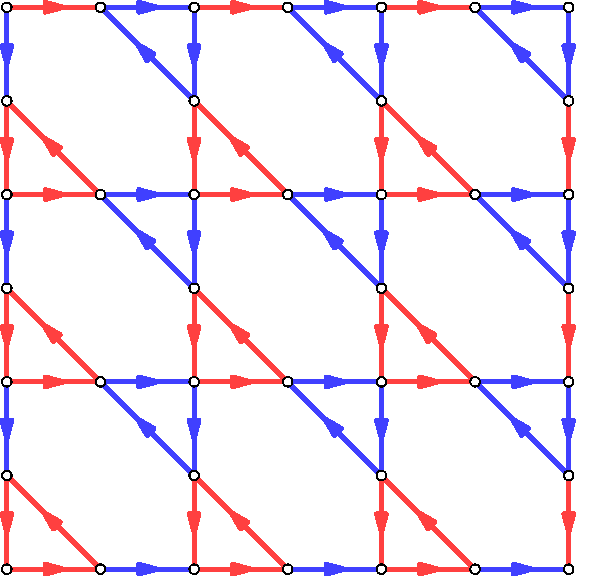
\includegraphics{C:/Users/jzchr/MathDocuments/Class Work/Topology/Homework/317HW2P3.pdf}
\end{figure}

The red and blue triangles indicate that $a^3,b^3$ are in this fundamental group, the hexagons give loops for $(ab^{-1})^3$, and the torus structure gives loops for $(ab)^3$.

In fact for any word $w$, $w^3$ is a loop: let $w$ be some word in $a,b,a^{-1},b^{-1}$. Since $a^2,a^{-1}$ have the same start and endpoints, we can consider the case where $w$ is just a string $a^{\pm}b^{\pm}a^{\pm}\dots b^{\pm}$. Geometrically, each $ab^{-1}$ or $b^{-1}a$ denotes a right turn while each $ba^{-1}$ or $a^{-1}b$ denotes a left turn, and $ab,a^{-1}b^{-1},ba,b^{-1}a^{-1}$ are straight. Thus each word $w$ has some ``net rotation'' that is either two right turns, two left turns, or straight (this is not hard to show). 

In the cases where $w$ is not straight, $w^3$ forms a path with threefold rotational symmetry, and is therefore a loop. When $w$ is straight, $w$ must have an even number of letters, so $w^3$ has a multiple of 6 letters, and thus it cycles around the torus to form a loop.
\end{proof}

\newpage 

\noindent \textbf{Problem 4 (Hatcher 1.3:18)}: For a space $X$ that is path-connected, locally path-connected, and semilocally simply-connected, call a covering space $\hat{X}\to X$ \textit{abelian} if it is normal and has abelian deck transformation group. Show that $X$ has a `universal' abelian covering space (i.e. one that covers every other abelian covering space of $X$) and it is unique up to isomorphism. Describe this covering space explicitly for $X=S^1\vee S^1$ and $X=S^1\vee S^1 \vee S^1$.

\begin{proof}
	The universal abelian covering space is the one whose fundamental group is the Abelianization of $\pi_1(X,x)$. The Deck transformation group is $\pi_1(X,x)/p_*(\pi_1(\hat{X},\hat{x}))$, and if this is Abelian then $p_*(\pi_1(\hat{X},\hat{x}))$ must include the commutator subgroup of $\pi_1(X,x)$, and in the maximal case it must be exactly the commutator subgroup.
	
	For $S^1\vee S^1$, the covering space is an infinite square grid, and the deck group is the translation group $\Z\times \Z$; for $S^1\vee S^1\vee S^1$ it is an infinite triangle grid.
	
\end{proof}

\newpage 

\noindent \textbf{Problem 5 (Hatcher 1.3:23)}: Show that if a group $G$ acts freely (no fixed points) and properly discontinuously (i.e. every $x\in X$ has a neighborhood $U$ with only finitely-many $g$ s.t. $U \cap g(U)\neq \emptyset$) on a Hausdorff space $X$, then the action is a covering space action.

\begin{proof}
	First, I claim that if $G$ acts on $X$ freely, then for every $g\in G$ and $x\in X$ there is some neighborhood $U_g$ of $x$ such that $x\not\in g(U_g)$. To get this neighborhood, let $V_1,V_2$ be neighborhoods of $x,g(x)$ which are disjoint ($X$ is Hausdorff) and take $U_g=V_1\cap g^{-1}(V_2)$.
	
	Using this fact, if $U$ is such that only finitely many a finite subset $G'\subset G$ has $g(U)\cap U\neq \emptyset$, then take the intersection of $U_g$ for $g\in G'$ to get a neighborhood $U_G$ of $x$ for which $x\not\in g(U_G)$ for any $g\in G$. Then by Hausdorff again, take a neighborhood $U'\subset U_G$ of $x$ disjoint from $g(U_G)$ for $g\in G'$, and thus for all $g\in G$. The fact that this $U'$ exists for all $x$ shows that $G$ is a covering space action.
	\end{proof}

\newpage 
\noindent \textbf{Problem 6 (Hatcher 1.3:25)}: Let $\ph:\R^2\to \R^2$ be the linear transformation $\ph(x,y) = (2x,y/2)$. Let $X:=\R^2-\{0\}$. $\Z$ acts on $X$ by $n: (x,y) \mapsto \ph^n(x,y)$. Show that this action is a covering space action and compute $\pi_1(X/\Z)$. Show that the orbit space $X/\Z$ is non-Hausdorff and describe how it is a union of four subspaces homeomorphic to $S^1\times \R$, coming from the complementary components of the $x$-axis and $y$-axis.

\begin{proof}
	First, this is a covering space action. One can check that the open square $(\tfrac12 x,2x)\times (\tfrac12 y,2y)$ is disjoint from its image under $\ph^n$ for $n\neq 0$.\\
	
	Knowing that this is a covering space action, it implies that $p:X\to X/\Z$ by $(x,y)\mapsto \ph^{\Z}(x,y)$ is a normal covering. And $X$ is both path-connected and locally path-connected, so we have
	$$
	\Z= \pi_1(X/\Z)/p_{*}(\pi_1(X)) = \pi_1(X/\Z)/\Z
	$$
	using the fact that $p_*(\Z)=\Z$, since $\ph$ has positive determinant and thus preserves orientation.
	This produces the short exact sequence
	$$
	1 \to \Z \to \pi_1(X/\Z) \to \Z\to 1
	$$
	which, because $\pi_1(X/\Z)$ is Abelian, is a splitting, which gives $\pi_1(X/\Z) = \Z^2$. To show that $\pi_1(X/\Z)$ is Abelian, it suffices to give two generators and show that they commute. These generators can be the projections of paths $\a,\b:[0,1]\to X$ given by 
	$$\a(t) = (\cos(t),\sin(t)) \,\, \text{ and } \,\, \b(t) = (t+1,0)$$
	($\b$ is a loop because $(1,0)\sim (2,0)$ mod the action of $\ph$). These commute up to homotopy, so the group is Abelian.\\
	
	$X/\Z$ is not Hausdorff: consider the points $(0,1)$ and $(1,0)$. If $U_1,U_2$ are any open neighborhoods of these points in $X$, then in $X/\Z$ they correspond to $\ph^{\Z}(U_1)$ and $\ph^{\Z}(U_2)$. Because these neighborhoods are open, for some $N\gg 0$, $U_1$ contains $(2^{-N},1)$ and $U_2$ contains $(1,2^{-N})$. But then $\ph^{N/2}(U_1)$ and $\ph^{-N/2}(U_2)$ both contain $(2^{-N/2},2^{-N/2})$. Thus, $U_1,U_2$ intersect in $X/\Z$.\\
	
	Finally, for every point $(x,y)\in X$ with $x>0$, we can find a unique representative of its equivalence class in $[1,2]\times \R$, with the right and left edges identified so that $(1,y)\sim (2,y/2)$, so that this part of $X/\Z$ is identified with $S^1\times \R$. Taking the union of these cylinders corresponding to the four half planes $x>0,y>0,x<0,y<0$ gives us the four components.
	
\end{proof}

\newpage 
\noindent \textbf{Problem 7 (Hatcher 1.A:6)}: Let $F$ be the free group on two generators and let $F'$ be its commutator subgroup. Find a set of free generators of $F'$ by considering the covering space of the graph corresponding to $F'$.

\begin{proof}
	One set of free generators is the commutators of the form $a^nb^ma^{-n}b^{-m}$ for $n,m\in \N$. The commutator subgroup is the fundamental group of the infinite square grid with $a$ on one axis and $b$ on the other. To find its generators, we can quotient by a maximal spanning tree. One such tree is the one consisting of the vertical line $x=0$ and the horizontal lines $y=n$ for $n\in \Z$. Upon taking the quotient, we get a wedge of infinitely-many loops, each of which is represented by an edge not present in the tree. These are exactly $a^nb^ma^{-n}b^{-m}$ for $n,m\in \N$.
\end{proof}

\newpage 
\noindent \textbf{Problem 8 (Hatcher 1.A:13)}: Let $x$ be a nontrivial element of a finitely-generated free group $F$. Show that there is a finite-index subgroup $H\subset F$ in which $x$ is part of a basis.

\begin{proof}
	Let $G$ be a graph whose fundamental group is $F$ (i.e. a wedge of finitely-many loops). $x$ is a product of these loops in some order. We can make a finite-sheeted covering space $\hat{G}$ which has $x$ as a loop; an example is shown for $x=ab^{-1}ccaaab$, but the same method will work in general:
	$$
	\begin{tikzcd}[sep=large]
		& \bullet & \bullet \\
		\bullet &&& \bullet \\
		\bullet &&& \bullet \\
		& \bullet & \bullet
		\arrow[color={rgb,255:red,92;green,214;blue,92}, from=1-2, to=1-2, loop, in=105, out=165, distance=5mm]
		\arrow["a", color={rgb,255:red,214;green,92;blue,92}, from=1-2, to=1-3]
		\arrow[color={rgb,255:red,92;green,214;blue,92}, from=1-3, to=1-3, loop, in=15, out=75, distance=5mm]
		\arrow["b", color={rgb,255:red,92;green,214;blue,214}, tail reversed, no head, from=1-3, to=2-4]
		\arrow["b"{description}, color={rgb,255:red,92;green,214;blue,214}, curve={height=12pt}, from=1-3, to=2-4]
		\arrow["b", color={rgb,255:red,92;green,214;blue,214}, from=2-1, to=1-2]
		\arrow["b"{description}, color={rgb,255:red,92;green,214;blue,214}, curve={height=12pt}, tail reversed, no head, from=2-1, to=1-2]
		\arrow[color={rgb,255:red,92;green,214;blue,92}, from=2-1, to=2-1, loop, in=105, out=165, distance=5mm]
		\arrow[color={rgb,255:red,214;green,92;blue,92}, from=2-4, to=2-4, loop, in=15, out=75, distance=5mm]
		\arrow["c", color={rgb,255:red,92;green,214;blue,92}, from=2-4, to=3-4]
		\arrow["c"{description}, color={rgb,255:red,92;green,214;blue,92}, curve={height=6pt}, tail reversed, no head, from=2-4, to=4-3]
		\arrow["a", color={rgb,255:red,214;green,92;blue,92}, from=3-1, to=2-1]
		\arrow[color={rgb,255:red,92;green,214;blue,214}, from=3-1, to=3-1, loop, in=150, out=210, distance=5mm]
		\arrow[color={rgb,255:red,92;green,214;blue,92}, from=3-1, to=3-1, loop, in=240, out=300, distance=5mm]
		\arrow[color={rgb,255:red,92;green,214;blue,214}, from=3-4, to=3-4, loop, in=330, out=30, distance=5mm]
		\arrow[color={rgb,255:red,214;green,92;blue,92}, from=3-4, to=3-4, loop, in=240, out=300, distance=5mm]
		\arrow["c", color={rgb,255:red,92;green,214;blue,92}, from=3-4, to=4-3]
		\arrow["a", color={rgb,255:red,214;green,92;blue,92}, from=4-2, to=3-1]
		\arrow[color={rgb,255:red,92;green,214;blue,92}, from=4-2, to=4-2, loop, in=240, out=300, distance=5mm]
		\arrow[color={rgb,255:red,92;green,214;blue,214}, from=4-2, to=4-2, loop, in=150, out=210, distance=5mm]
		\arrow["a"{description}, color={rgb,255:red,214;green,92;blue,92}, curve={height=6pt}, tail reversed, no head, from=4-3, to=2-1]
		\arrow["a", color={rgb,255:red,214;green,92;blue,92}, from=4-3, to=4-2]
		\arrow[color={rgb,255:red,92;green,214;blue,214}, from=4-3, to=4-3, loop, in=285, out=345, distance=5mm]
	\end{tikzcd}
	$$
	
	The fundamental group $p_*(\pi_1(\hat{G}))\subset G$ will be a finite index subgroup (because the covering has finitely-many sheets) and has $x$ as part of a basis because it is a loop in $\hat{G}$ (one can take a maximal spanning tree consisting of all but one edge in the loop representing $x$).
\end{proof}

\end{document}